\documentclass[12pt]{article}
\usepackage{float}
\usepackage{graphicx}
\usepackage[font=small,labelfont=bf]{caption}
\usepackage{xcolor}

\pagestyle{empty}
\setcounter{tocdepth}{4}
\setcounter{secnumdepth}{4}

\topmargin=0cm
\oddsidemargin=0cm
\textheight=22.0cm
\textwidth=16cm
\parindent=0cm
\parskip=0.15cm
\topskip=0truecm
\raggedbottom
\abovedisplayskip=3mm
\belowdisplayskip=3mm
\abovedisplayshortskip=0mm
\belowdisplayshortskip=2mm
\normalbaselineskip=12pt
\normalbaselines

\begin{document}

\definecolor{light-gray}{gray}{0.95}
\newcommand{\code}[1]{\colorbox{light-gray}{\texttt{#1}}}

\vspace*{0.5in}
\centerline{\bf\Large Design Document - Iteration 2}

\vspace*{0.5in}
\centerline{\bf\Large Team PA-PI-a}

\vspace*{0.5in}
\centerline{\bf\Large 18 March 2018}

\vspace*{1.5in}
\begin{table}[htbp]
\caption{Team}
\begin{center}
\begin{tabular}{|r | c|}
\hline
Name & ID Number \\
\hline\hline
Melanie Taing & 40009850 \\
Laurie Gagnon & 22943433 \\
Wayne Yiel Leung & 26586988 \\
Jordan Rutty & 27300107 \\
Alice Barkhouse & 27486782 \\
Michael Foo & 40000225 \\
Pierre-Andre Leger & 40004010 \\
Colin Greczkowski & 40001600 \\
\hline
\end{tabular}
\end{center}
\end{table}

\clearpage

\tableofcontents
\clearpage

\listoffigures
\clearpage

\section{Introduction}
The purpose of this document is to describe and provide details for the design and
implementation of the second iteration of the MyMoney application.\\

The following pages will cover the rational of the architectural design as well as the
subsystem interface specifications and details on their implementation. Finally, we will
describe three dynamic design scenarios based on use cases specified in the documentation
for iteration 1.

\section{Architectural Design} \label{sec:arch}
The Mymoney application is implemented using a model-view-controller (MVC) architecture. this section will cover the architectural diagram for the MVC as well as the subsystem interface specifications.
\newpage
\subsection{Architectural Diagram}

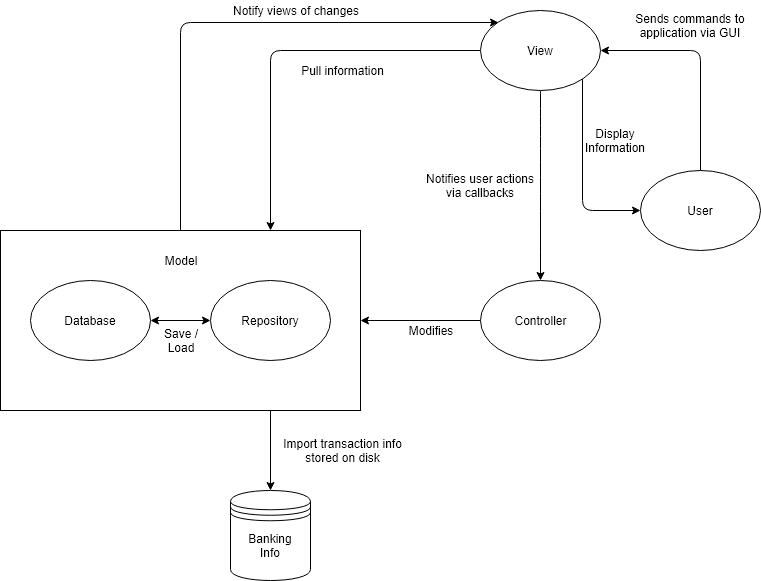
\includegraphics[width=\textwidth,height=\textheight,keepaspectratio]{diagrams/UML/MVC.png}
\captionof{figure}{High level structure of MVC architecture}\bigskip
The model contains all the information related to the transactions and the accounts that the user wishes to track. It consists of an SQL database used to serialize and deserialize   the information between user sessions and a repository with which the rest of the application interacts. Modifications to the repository are saved on-the-fly to the database while the program is running. The view displays the accounts and transactions loaded into the model (repository) and offers interactive elements that the user can interact with. In essence, it is a GUI. The controller handles user input from the view (GUI) and then acts on the model accordingly by adding, modifying or deleting transactions or accounts.\\

The main advantage of using an MVC pattern is the separation of concerns. As will be demonstrated in the next section, by enforcing each subsystem to depend strictly on \code{Interface} types when communicating with each other, we can reduce dependencies and greatly increase modularity.



\subsection{Subsystem Interface Specifications}

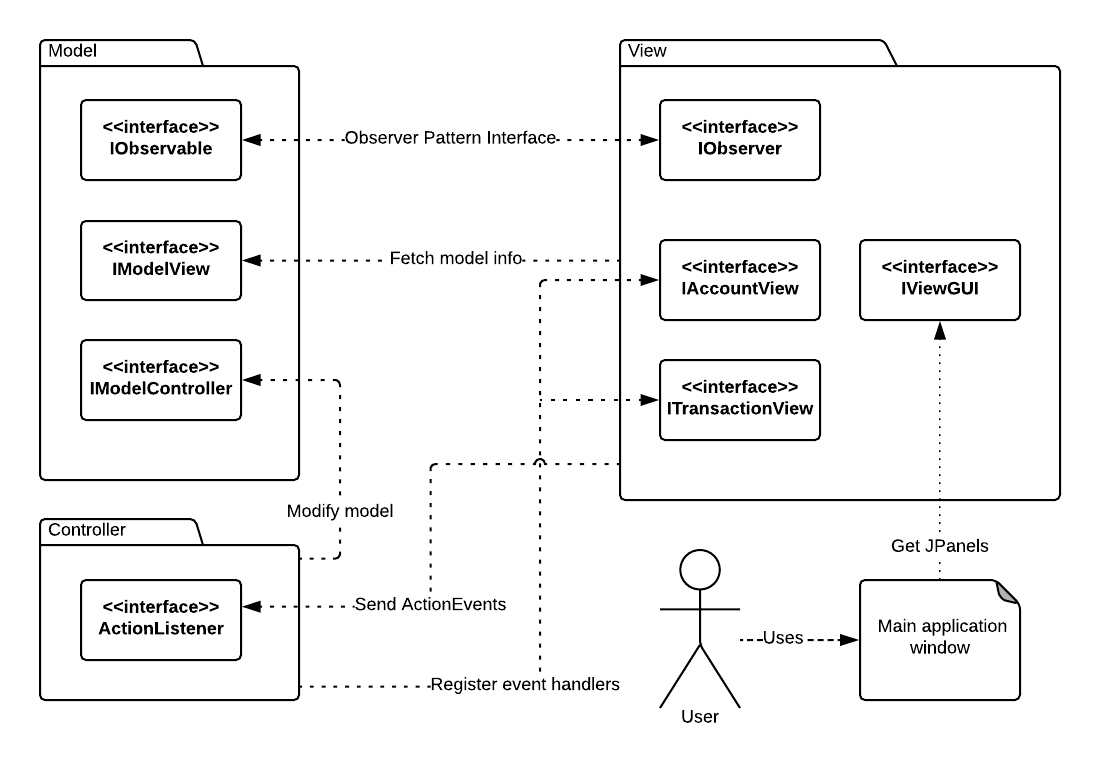
\includegraphics[width=\textwidth,height=\textheight,keepaspectratio]{diagrams/UML/Subsystem.png}
\captionof{figure}{Subsystem specification diagram}\bigskip

\subsubsection{Model - View : Observer Pattern}
The interfaces \code{IObservable} and \code{IObserver} form the observer pattern between the model and the view.\\

\code{IObserver}
\begin{itemize}
	\item \code{update()} : Called by an \code{IObservable} object. This should trigger internal logic in the observer to allow it to update its view on the model.
\end{itemize}\bigskip

\code{IObservable}
\begin{itemize}
	\item \code{attachObserver(IObserver)} : Attach an observer to this object
	\item \code{detachObserver(IObserver)} : Detach an observer from this object
	\item \code{notifyObservers()} : Call the \code{update()} method on all attached observers. Whenever the state of the model changes, it should call this function to allow its attached observers to update their views.
\end{itemize}\bigskip

\subsubsection{Model : IModelView Interface}
The \code{ImodelView} interface exposes methods to allow the view to fetch information from the the model.\\
\begin{itemize}
	\item \code{getTransactions(Integer accountId)} : Returns a list of \code{Transaction} objects belonging to the specified accountId. If there are no transactions for the account or the account does not exist, it will return an empty list.
	\item \code{getAllAccounts()} : Returns a list of all the \code{Account} objects for the current user.
\end{itemize}

\subsubsection{Model : IModelController Interface}
The \code{IModelController} interface exposes methods to allow the controller to modify the model.\\
\begin{itemize}
	\item \code{saveTransaction(Transaction)} : Save the given \code{Transaction} object to the repository and update the SQL database. If the ID of the transaction is 0, create a new entry. Otherwise update the existing one.
	\item \code{saveAccount(Account)} : Save the given \code{Account} object to the repository and update the SQL database. If the ID of the account is 0, create a new entry. Otherwise update the existing one.
	\item \code{deleteTransaction(Transaction)} : Delete the specified transaction from both the repository and the SQL database.
	\item \code{deleteAccount(Account)} : Delete the specified account from both the repository and the SQL database.
	\item \code{importTransactions(String path, Integer accountId)} : Construct and save \code{Transactions} objects to the repository and SQL databse from a .csv file located at the specified path. The format of the .csv file should be well defined.
\end{itemize}

\subsubsection{View : IAccountView}
The \code{IAccountView} interface exposes methods to allow the controller to register event listeners for user actions (buttons clicks) and have access to the content of the form fields filled by the user.\\
The callback system uses Java's \code{ActionEvent} class. 
\begin{itemize}
	\item \code{registerAddActionCallback(ActionListener, String)} : Attach the specified listener to the GUI element that should trigger the "Add" action and set the event's action command to the specified string (should be "Add").
	\item \code{registerUpdateActionCallback(ActionListener, String)} : Attach the specified listener to the GUI element that should trigger the "Update" action and set the event's action command to the specified string (should be "Update").
	\item \code{registerDeleteActionCallback(ActionListener, String)} : Attach the specified listener to the GUI element that should trigger the "Delete" action and set the event's action command to the specified string (should be "Delete").
	\item \code{getBankInput()} : Return a string consisting of the content of the BankName field in the GUI.
	\item \code{getNicknameInput()} : Return a string consisting of the content of the Nickname field in the GUI.
	\item \code{getBalanceInput()} : Return an Integer consisting of the content of the Balance field in the GUI.
	\item \code{getSelectedAccountId()} : Return a Integer consisting of the id of the account currently selected by the user.
	\item \code{setSelection(Integer)} : Overrides the user's current account selection. This method mostly improves user experience (for example, automatically selects a new account when it is created)
\end{itemize}

\subsubsection{View : ITransactionView}
The \code{ITransactionView} interface exposes methods to allow the controller to register event listeners for user actions (buttons clicks) and have access to the content of the form fields filled by the user.\\
The callback system uses Java's \code{ActionEvent} class.
\begin{itemize}
	\item \code{registerAddActionCallback(ActionListener, String)} : Attach the specified listener to the GUI element that should trigger the "Add" action and set the event's action command to the specified string (should be "Add").
	\item \code{registerUpdateActionCallback(ActionListener, String)} : Attach the specified listener to the GUI element that should trigger the "Update" action and set the event's action command to the specified string (should be "Update").
	\item \code{registerDeleteActionCallback(ActionListener, String)} : Attach the specified listener to the GUI element that should trigger the "Delete" action and set the event's action command to the specified string (should be "Delete").
		\item \code{registerImportActionCallback(ActionListener, String)} : Attach the specified listener to the GUI element that should trigger the "Import" action and set the event's action command to the specified string (should be "Import").
	\item \code{getTypeInput()} : Return a string consisting of the content of the Type field in the GUI.
	\item \code{getDateInput()} : Return a string consisting of the content of the Date field in the GUI.
	\item \code{getDescriptionInput()} : Return a string consisting of the content of the Description field in the GUI.
	\item \code{getAmountInput()} : Return an Integer consisting of the content of the Amount field in the GUI.
	\item \code{getSelectedAccountId()} : Return a Integer consisting of the id of the account currently selected by the user.
	\item \code{getSelectedTransactionId()} : Return a Integer consisting of the id of the transaction currently selected by the user.
	\item \code{setSelection(Integer)} : Overrides the user's current transaction selection. This method mostly improves user experience (for example, resetting the current selection when a transaction is deleted)
\end{itemize}

\subsubsection{View : IViewGUI}
The \code{IViewGUI} interface exposes a single method that returns a \code{JPanel} object. It is only used by the main application window.
\begin{itemize}
	\item \code{getPanel()} : Returns the topmost parent \code{JPanel} of this view. It is meant to be used by the main application window to populate its frame.
\end{itemize}

\subsubsection{Controller : ActionListener}
The controller only needs to listen to events triggered by the user's input. From the other subsystems' perspective, it implements a single interface with a single method.
\begin{itemize}
	\item \code{actionPerformed(ActionEvent)} : Event handler for \code{ActionEvent} events created by the view. The controller registers its handlers by using the \code{IAccountView} or \code{ITransactionView} interfaces provided by the view(s).
\end{itemize}








\section{Detailed Design} \label{sec:detail}

\textit {From the template (delete me) --- Complete description of the system design, describing one subsystem separately in respective subsection. UML class diagrams are to be used, as well as a short textual description describing the purpose of each class.}

\subsection{Subsystem X}

\subsubsection{Detailed Design Diagram}

\textit {From the template (delete me) --- UML class diagram depicting the internal structure of the subsystem, accompanied by a paragraph of text describing the rationale of this design.}

\subsubsection{Units Description}


\paragraph {AbstractAppController.java}
\begin{center}
\footnotesize
\begin{tabular}{|l|l|}
\hline
\textbf{Class Name }   & {AbstractAppController.java} \\ \hline
\textbf {Inherits} & {~} \\ \hline
\textbf {Description}   & {Abstract App Controller} \\ \hline
\textbf {Attributes} & ~ \\ \hline
\textbf {Methods} & 

\footnotesize
\begin{tabular}{l|l|l|l}
\textbf{Visibility} & \textbf{Method Name} & \textbf{Return type} &\textbf{Description} \\ \hline
public &AbstractAppController &~&Constructor\\ \hline
public &start &void &Abstract start class\\ \hline
public &shutdown&void &Abstract shutdown class\\ \hline
public &run &void &Abstract run class\\
\end{tabular} \\ \hline

\end{tabular}
\end{center}

\paragraph {AbstractEventListener.java}
\begin{center}
\footnotesize
\begin{tabular}{|l|l|}
\hline
\textbf {Class Name} & {AbstractEventListener.java} \\ \hline 
\textbf {Inherits} & { java.awt.event.ActionListener} \\ \hline 
\textbf {Description} & { Abstract Event Listener} \\ \hline 
\textbf {Attributes} &

\footnotesize
\begin{tabular}{l|l|l|l}
\textbf{Visibility} & \textbf{Data type} & \textbf{Name} & \textbf{Description} \\ \hline
package& AbstractView & view & ~  \\ \hline
package & AbstractViewController & controller & ~
\end{tabular} \\ \hline
\textbf {Methods} &

\footnotesize
\begin{tabular}{l|l|l|p{3.0cm}}
\vspace*{0.1cm}
\textbf{Visibility} & \textbf{Method Name} & \textbf{Return type} &\textbf{Description} \\ \hline
public &AbstractEventListener&~ &Constructor \\ \hline 
public &setView &void&Setter for view \\ \hline 
public &getView &AbstractView &Getter for view \\ \hline 
public&setController &void&Setter for controller \\ \hline 
public &getController&AbstractViewController&Getter for controller \\ \hline 
public &actionPerformed&void&Default message to implement this method in the view controller

\end{tabular} \\ \hline

\end{tabular}
\end{center}

\paragraph {AbstractModel.java}
\begin{center}
\footnotesize
\begin{tabular}{|l|l|}
\hline
\textbf {Class Name} & {AbstractModel.java} \\ \hline 
\textbf {Inherits} & {} \\ \hline 
\textbf {Description} & { Abstract class for models} \\ \hline 
\textbf {Attributes} &

\footnotesize
\begin{tabular}{l|l|l|l}
\textbf{Visibility} & \textbf{Data type} & \textbf{Name} & \textbf{Description} \\ \hline
package&boolean &boolNew&used to determine if id has been set \\ \hline
private & HashSet\textless AbstractView\textgreater & m\textunderscore views & stores the views \\
\end{tabular} \\ \hline
\textbf {Methods} &

\footnotesize
\begin{tabular}{l|l|l|l}
\textbf{Visibility} & \textbf{Method Name} & \textbf{Return type} &\textbf{Description} \\ \hline
public &isNew&boolean &getter for boolNew \\ \hline 
public &setIsNewModel&void&setter for boolNew \\ \hline 
public &setView &void &setter for views \\ \hline 
public &removeView &void &deletes views \\ \hline 
public &notifyViews&void &calls for update on all views
\end{tabular} \\ \hline

\end{tabular}
\end{center}

\paragraph {AbstractView.java}
\begin{center}
\footnotesize
\begin{tabular}{|l|l|}
\hline
\textbf {Class Name} & {AbstractView.java} \\ \hline 
\textbf {Inherits} & {} \\ \hline 
\textbf {Description} & { Abstract view class} \\ \hline 
\textbf {Attributes} & ~ \\ \hline
\textbf {Methods} &

\footnotesize
\begin{tabular}{l|l|l|l}
\textbf{Visibility} & \textbf{Method Name} & \textbf{Return type} &\textbf{Description} \\ \hline
package&AbstractView &Constructor \\ \hline 
public&update &void&abstract update class
\end{tabular} \\ \hline

\end{tabular}
\end{center}
\paragraph {AbstractViewController.java}
\begin{center}
\footnotesize
\begin{tabular}{|l|l|}
\hline
\textbf {Class Name} & {AbstractViewController.java} \\ \hline 
\textbf {Inherits} & {} \\ \hline 
\textbf {Description} & { Abstract class for view controller} \\ \hline 
\textbf {Attributes} &

\footnotesize
\begin{tabular}{l|l|l|p{5.8cm}}
\textbf{Visibility} & \textbf{Data type} & \textbf{Name} & \textbf{Description} \\ \hline
package &AbstractView &view &primary view \\ \hline 
package &AbstractView &secondaryView&secondary view \\ \hline 
private &boolean &controllerInitialized&determines if the controller has been initialized
\end{tabular} \\ \hline
\textbf {Methods} &

\footnotesize
\begin{tabular}{l|l|l|l}
\textbf{Visibility} & \textbf{Method Name} & \textbf{Return type} &\textbf{Description} \\ \hline
public&AbstractViewController&~&constructor \\ \hline 
public&setView&void&Setter for view \\ \hline 
public&getView&AbstractView &Getter for view \\ \hline 
public&setSecondaryView&void&Setter for secondary view \\ \hline 
public&getSecondaryView&AbstractView &Getter for secondary view \\ \hline 
public&setIsInitialized&void&Setter for controllerInitialized \\ \hline 
public&getIsInitialized&boolean&getter for controllerInitialized
\end{tabular} \\ \hline

\end{tabular}
\end{center}
\paragraph {AccountController.java}
\begin{center}
\footnotesize
\begin{tabular}{|l|l|}
\hline
\textbf {Class Name} & {AccountController.java} \\ \hline 
\textbf {Inherits} & { AbstractViewController} \\ \hline 
\textbf {Description} & { Controller for the accounts, initializing all the form elements associated to account} \\ \hline 
\textbf {Attributes} &

\footnotesize
\begin{tabular}{l|l|l|l}
\textbf{Visibility} & \textbf{Data type} & \textbf{Name} & \textbf{Description} \\ \hline
private &UserModel&user &user model object
\end{tabular} \\ \hline
\textbf {Methods} &

\footnotesize
\begin{tabular}{l|l|l|p{3cm}}
\textbf{Visibility} & \textbf{Method Name} & \textbf{Return type} &\textbf{Description} \\ \hline
protected&AccountController &~&Constructor \\ \hline 
protected &initController &void&binds event listeners/controls to all account view elements and populates form data \\ \hline 
public &setUser &void &setter for user \\ \hline 
public &getUser &UserModel &getter for user \\ \hline 
private &addButton &void &Behaviour of the "add account" button \\ \hline 
private &updateButton&void &Behaviour of the "update account" button \\ \hline 
private &deleteButton &void &Behaviour of the "delete account" button \\ \hline 
private &clearButton &void &Behaviour of the "clear" button \\ \hline 
protected &getAccountDataFromAddAccountInput&AccountModel&add data inputs to account model \\ \hline 
private &resetAddAccountInput &void &clear the UI account inputs \\ \hline 
public &getAccountDataFromRow&AccountModel&Given a row number, get account data \\ \hline 
protected &updateDataRowFromModel&void &modify account data given UI input \\ \hline 
public &update &void &Update the attached models
\end{tabular} \\ \hline

\end{tabular}
\end{center}


\paragraph {AccountModel.java}
\begin{center}
\footnotesize
\begin{tabular}{|l|l|}
\hline
\textbf {Class Name} & {AccountModel.java} \\ \hline 
\textbf {Inherits} & { AbstractModel} \\ \hline 
\textbf {Description} & { Model for bank accounts} \\ \hline 
\textbf {Attributes} &

\footnotesize
\begin{tabular}{l|p{3cm}|l|p{6cm}}
\textbf{Visibility} & \textbf{Data type} & \textbf{Name} & \textbf{Description} \\ \hline
private&int &accountId &the Id of the account \\ \hline 
private&String &bankName &the name of the bank the account is held with \\ \hline 
private&String &nickName &the nickname for the account \\ \hline 
private&int &balance &the dollar balance of the account \\ \hline 
package &AccountTransaction-\newline Repository&transactionsRepo &repository that holds account transaction information
\end{tabular} \\ \hline
\textbf {Methods} &

\footnotesize
\begin{tabular}{l|p{3.5cm}|p{3.5cm}|p{4.5cm}}
\textbf{Visibility} & \textbf{Method Name} & \textbf{Return type} &\textbf{Description} \\ \hline
public &AccountModel &Constructor\\ \hline 
public &hasId &boolean &determines if an account has an Id\\ \hline 
public &getId &int &getter for Id\\ \hline 
public &setId &void &setter for Id\\ \hline 
public &hasBankName&boolean &determines if an account has a bank name\\ \hline 
public &getBankName&String &getter for bank name\\ \hline 
public &setBankName &void &setter for bank name\\ \hline 
public &hasNickName&boolean &determines if an account has a nick name\\ \hline 
public &getNickName&String &getter for nick name\\ \hline 
public &setNickName &void &setter for nick name\\ \hline 
public &hasBalance&boolean &determines if an account has a balance\\ \hline 
public &getBalance&int &getter for balance\\ \hline 
public &setBalance&void &setter for balance\\ \hline 
public &toString &String &generates a formatted output of all the account details\\ \hline 
public &setAccount-\newline TransactionRepository&void &Setter for transactionsRepo\\ \hline 
public &getAccount-\newline TransactionRepository&AccountTransaction-\newline Repository &Getter for transactionsRepo\\ \hline 
public &getMapOf-\newline AllTransactions &TransactionMap&gets map of all transactions\\ \hline 
public &getListOfAll-\newline Transactions &TransactionList&gets list of all transactions\\ \hline 
public &saveTransaction&void &Saves a transaction to the repository\\ \hline 
public &deleteTransaction&void &deletes a transaction from the repository
\end{tabular} \\ \hline

\end{tabular}
\end{center}
\paragraph {AccountRepository.java}
\begin{center}
\footnotesize
\begin{tabular}{|l|l|}
\hline
\textbf {Class Name} & {AccountRepository.java} \\ \hline 
\textbf {Inherits} & {} \\ \hline 
\textbf {Description} & { Provides functionality to a user's bank accounts database} \\ \hline 
\textbf {Attributes} &

\footnotesize
\begin{tabular}{l|l|l|l}
\textbf{Visibility} & \textbf{Data type} & \textbf{Name} & \textbf{Description} \\ \hline
package&Database &myDatabase &Database that stores account information\\ \hline 
package&SQLStringFactory &sql &Builds valid SQL statements\\ \hline 
package &String &tableName &Name of the table\\ \hline 
package &String &primaryKey &Name of the databases' primary key\\ \hline 
package &Boolean &boolAllLoaded &Have all accounts been loaded in database?\\ \hline 
package &AccountMap &itemMap&holds loaded account models
\end{tabular} \\ \hline
\textbf {Methods} &

\footnotesize
\begin{tabular}{l|l|l|l}
\textbf{Visibility} & \textbf{Method Name} & \textbf{Return type} &\textbf{Description} \\ \hline
public &AccountRepository &~&Constructor\\ \hline 
protected &hasItemCached&boolean &checks if item is in itemMap\\ \hline 
public &saveItem&void &Save or update an account\\ \hline 
public&deleteItem&void&Deletes an account\\ \hline 
public &getItem&AccountModel&getter for account item\\ \hline 
public &getMapOfAllItems&AccountMap&getter for map of all items\\ \hline 
public&getListOfAllItems&AccountList&getter for all items\\ \hline 
protected &loadItem&void&load an account\\ \hline 
protected&loadAll&void&load all accounts\\ \hline 
protected&setItemFromResult&void&populate the model with account information\\ \hline 
protected&addItemToMap&void&Add an account to the item map
\end{tabular} \\ \hline

\end{tabular}
\end{center}
\paragraph {AccountTransactionRepository.java}
\begin{center}
\footnotesize
\begin{tabular}{|l|l|}
\hline
\textbf {Class Name} & {AccountTransactionRepository.java} \\ \hline 
\textbf {Inherits} & { TransactionRepository} \\ \hline 
\textbf {Description} & { Contains access to all of the transactions for an account} \\ \hline 
\textbf {Attributes} &

\footnotesize
\begin{tabular}{l|l|l|p{8cm}}
\textbf{Visibility} & \textbf{Data type} & \textbf{Name} & \textbf{Description} \\ \hline
package&AccountModel&account &The account object from which we are accessing transactions
\end{tabular} \\ \hline
\textbf {Methods} &

\footnotesize
\begin{tabular}{l|p{3.5cm}|l|l}
\textbf{Visibility} & \textbf{Method Name} & \textbf{Return type} &\textbf{Description} \\ \hline
public&AccountTransaction-\newline Repository&~&Constructor\\ \hline 
public&setAccount&void&Setter for account\\ \hline 
public&getAccount&AccountModel&Getter for account\\ \hline 
public&hasAccount&boolean &Check if account has been initialized\\ \hline 
public &loadAllItems&void&load all transactions for account\\ \hline 
public &saveItem&void&Save a transaction to account
\end{tabular} \\ \hline

\end{tabular}
\end{center}
\paragraph {AccountView.java}
\begin{center}
\footnotesize
\begin{tabular}{|l|l|}
\hline
\textbf {Class Name} & {AccountView.java} \\ \hline 
\textbf {Inherits} & { AbstractView} \\ \hline 
\textbf {Description} & { The view for accounts (accounts UI)} \\ \hline 
\textbf {Attributes} &

\footnotesize
\begin{tabular}{l|l|l|l}
\textbf{Visibility} & \textbf{Data type} & \textbf{Name} & \textbf{Description} \\ \hline
private &JPanel &panel&Various account UI elements\\ \hline 
private &DefaultTableModel &model &...\\ \hline 
private &JLabel &accLabel\\ \hline 
private &JLabel &accountIDLabel\\ \hline 
private &JLabel &bankLabel\\ \hline 
private &JLabel &nicknameLabel\\ \hline 
private &JLabel &balanceLabel\\ \hline 
private &JButton &addButton\\ \hline 
private &JButton &updateButton\\ \hline 
private &JButton &deleteButton\\ \hline 
private &JButton &clearButton\\ \hline 
private &JTextField &accountIDTextfield\\ \hline 
private &JTextField &bankTextfield\\ \hline 
private &JTextField &nicknameTextfield\\ \hline 
private &JTextField &balanceTextfield\\ \hline 
private &JTable &table\\ \hline 
private &JScrollPane &scrollPane&
\end{tabular} \\ \hline

\end{tabular}
\end{center}
\begin{center}
\footnotesize
\begin{tabular}{|l|l|}
\hline
\textbf {Methods} &

\footnotesize
\begin{tabular}{l|l|l|p{5cm}}
\textbf{Visibility} & \textbf{Method Name} & \textbf{Return type} &\textbf{Description} \\ \hline
public  &getPanel&JPanel&getter for panel\\ \hline 
public  &setPanel&void&setter for panel\\ \hline 
public  &getTableModel&DefaultTableModel&getter for table model\\ \hline 
public  &setTableModel&void&setter for table model\\ \hline 
public  &getAccLabel&JLabel&getter for account label\\ \hline 
public  &setAccLabel&void&setter for account label\\ \hline 
public  &getAccountIDLabel&JLabel&getter for account id label\\ \hline 
public  &setAccountIDLabel&void&setter getter account id label\\ \hline 
public  &getBankLabel&JLabel&getter for bank label\\ \hline 
public  &setBankLabel&void&setter for bank label\\ \hline 
public  &getNicknameLabel&JLabel&getter for nickname label\\ \hline 
public  &setNickname&void&setter for nickname label\\ \hline 
public  &getBalanceLabel&JLabel&getter for balance label\\ \hline 
public  &setBalanceLabel&void&setter for balance label\\ \hline 
public  &getAccountIDTextfield&JTextField&getter for account id textfield\\ \hline 
public  &setAccountIDTextfield&void&setter for account id textfield\\ \hline 
public  &getBankTextfield&JTextField&getter for bank textfield\\ \hline 
public  &setBankTextfield&void&setter for bank textfield\\ \hline 
public  &getNicknameTextfield&JTextField&getter for nickname textfield\\ \hline 
public  &setNicknameTextfield&void&setter for nickname textfield\\ \hline 
public  &getBalanceTextfield&JTextField&getter for balance textfield\\ \hline 
public  &setBalanceTextfield&void&setter for balance textfield\\ \hline 
public  &getAddButton&Button&getter for add button\\ \hline 
public  &setAddButton&void&setter for add button\\ \hline 
public  &getUpdateButton&JButton&getter for update button\\ \hline 
public  &setUpdateButton&void&setter for update button\\ \hline 
public  &getDeleteButton&JButton&getter for delete button\\ \hline 
public  &setDeleteButton&void&setter for delete button\\ \hline 
public  &getClearButton&JButton&getter for clear button\\ \hline 
public  &setClearButton&void&setter for clear button\\ \hline 
public  &getTable&JTable&getter for table\\ \hline 
public  &setTable&void&setter for table\\ \hline 
public  &getScrollPane&JScrollPane&getter for scroll pane\\ \hline 
public  &setScrollPane&void&setter for scroll pane\\ \hline 
public &update &void &updates the Jtable\\ \hline 
private &createAccPanel &void &creates the account UI elements\\ \hline 
private &setLayout &void &sets the visuals and grouping of the UI layout
\end{tabular} \\ \hline

\end{tabular}
\end{center}
\paragraph {Database.java}
\begin{center}
\footnotesize
\begin{tabular}{|l|l|}
\hline
\textbf {Class Name} & {Database.java} \\ \hline 
\textbf {Inherits} & {} \\ \hline 
\textbf {Description} & { The database object for storing/retrieving/altering data in the various databases.} \\ \hline 
\textbf {Attributes} &

\footnotesize
\begin{tabular}{l|l|l|l}
\textbf{Visibility} & \textbf{Data type} & \textbf{Name} & \textbf{Description} \\ \hline
private&String &m\textunderscore driver& database driver\\ \hline 
private&String &m\textunderscore dbName& database name\\ \hline 
private&Connection &m\textunderscore connection& connection to database
\end{tabular} \\ \hline
\textbf {Methods} &

\footnotesize
\begin{tabular}{l|l|l|l}
\textbf{Visibility} & \textbf{Method Name} & \textbf{Return type} &\textbf{Description} \\ \hline
public&Database &    &Constructor\\ \hline 
public&getConnection &Connection &Getter for connection\\ \hline 
public&fetchSQL&ResultSet &Executes an SQL query\\ \hline 
public &updateSQL &Integer &Executes an SQL update\\ \hline 
public &shutdown&void&Terminates connection
\end{tabular} \\ \hline

\end{tabular}
\end{center}
\paragraph {DummyAppController.java}
\begin{center}
\footnotesize
\begin{tabular}{|l|l|}
\hline
\textbf {Class Name} & {DummyAppController.java} \\ \hline 
\textbf {Inherits} & { AbstractAppController} \\ \hline 
\textbf {Description} & { Controller for a dummy app} \\ \hline 
\textbf {Attributes} &

\footnotesize
\begin{tabular}{l|l|l|l}
\textbf{Visibility} & \textbf{Data type} & \textbf{Name} & \textbf{Description} \\ \hline
package &Database &myDatabase &the database where app data is stored\\ \hline 
package&SQLStringFactory &sql &Builds valid SQL statements
\end{tabular} \\ \hline
\textbf {Methods} &

\footnotesize
\begin{tabular}{l|l|l|l}
\textbf{Visibility} & \textbf{Method Name} & \textbf{Return type} &\textbf{Description} \\ \hline
public &DummyAppController &~&Constructor\\ \hline 
public &start &void &starts the app\\ \hline 
public &run &void &initialize and run the dummy app
\end{tabular} \\ \hline

\end{tabular}
\end{center}
\paragraph {ImportTransaction.java}
\begin{center}
\footnotesize
\begin{tabular}{|l|l|}
\hline
\textbf {Class Name} & {ImportTransaction.java} \\ \hline 
\textbf {Inherits} & {} \\ \hline 
\textbf {Description} & { Imports transaction data from a CSV file} \\ \hline 
\textbf {Attributes} &

\footnotesize
\begin{tabular}{l|p{3cm}|p{3cm}|p{5.5cm}}
\textbf{Visibility} & \textbf{Data type} & \textbf{Name} & \textbf{Description} \\ \hline
package&String &transactionFilePath&the filepath of the csv that holds new transaction data\\ \hline 
private &AccountTransaction-\newline Repository &accountTransaction-\newline Repository &the repository that holds transaction data
\end{tabular} \\ \hline
\textbf {Methods} &

\footnotesize
\begin{tabular}{l|p{4cm}|l|p{5.5cm}}
\textbf{Visibility} & \textbf{Method Name} & \textbf{Return type} &\textbf{Description} \\ \hline
public &setAccount-\newline TransactionRepository&void&setter for accountTransactionRepository\\ \hline 
public&addTransaction&void &Imports transactions from CSV and stores in repository
\end{tabular} \\ \hline

\end{tabular}
\end{center}
\paragraph {Iteration2AppController.java}
\begin{center}
\footnotesize
\begin{tabular}{|l|l|}
\hline
\textbf {Class Name} & {Iteration2AppController.java} \\ \hline 
\textbf {Inherits} & {} \\ \hline 
\textbf {Description} & App controller for current project iteration \\ \hline 
\textbf {Attributes} &

\footnotesize
\begin{tabular}{l|l|l|p{4.5cm}}
\textbf{Visibility} & \textbf{Data type} & \textbf{Name} & \textbf{Description} \\ \hline
package &Database &myDatabase &the database where app data is stored\\ \hline 
package&SQLStringFactory &sql &Builds valid SQL statements\\ \hline 
package &AccountRepository &theAccountRespository&the repository that holds account data\\ \hline 
package &TransactionRepository &theTransactionRepository&the repository that holds transaction data
\end{tabular} \\ \hline
\textbf {Methods} &

\footnotesize
\begin{tabular}{l|l|l|p{6cm}}
\textbf{Visibility} & \textbf{Method Name} & \textbf{Return type} &\textbf{Description} \\ \hline
public &Iteration2AppController&~&Constructor\\ \hline 
public &start &void &starts the app\\ \hline 
protected&devStart &void &starts the app in development mode\\ \hline 
protected&productionStart &void &starts the app in production mode\\ \hline 
protected&InsertFakeAccounts &void &Adds some generic data to accounts repository for development\\ \hline 
public &run &void&initializes and runs the i2 app
\end{tabular} \\ \hline

\end{tabular}
\end{center}

\paragraph {MainController.java}
\begin{center}
\footnotesize
\begin{tabular}{|l|l|}
\hline
\textbf {Class Name} & {MainController.java} \\ \hline 
\textbf {Inherits} & { AbstractViewController} \\ \hline 
\textbf {Description} & { The main controller for the app} \\ \hline 
\textbf {Attributes} &

\footnotesize
\begin{tabular}{l|l|l|p{7cm}}
\textbf{Visibility} & \textbf{Data type} & \textbf{Name} & \textbf{Description} \\ \hline
package &UserModel &user &the user of the app
\end{tabular} \\ \hline
\textbf {Methods} &

\footnotesize
\begin{tabular}{l|l|l|p{6cm}}
\textbf{Visibility} & \textbf{Method Name} & \textbf{Return type} &\textbf{Description} \\ \hline
public &MainController &~&Constructor\\ \hline 
public &setUser &void &Setter for user\\ \hline 
public &getUser &UserModel &Getter for user\\ \hline 
public &initController &void &initialized the account, transaction and main view
\end{tabular} \\ \hline

\end{tabular}
\end{center}
\paragraph {MainView.java}
\begin{center}
\footnotesize
\begin{tabular}{|l|l|}
\hline
\textbf {Class Name} & {MainView.java} \\ \hline 
\textbf {Inherits} & { AbstractView} \\ \hline 
\textbf {Description} & { The main view for the app} \\ \hline 
\textbf {Attributes} &

\footnotesize
\begin{tabular}{l|l|l|l}
\textbf{Visibility} & \textbf{Data type} & \textbf{Name} & \textbf{Description} \\ \hline
protected &JFrame &mainFrame &Swing framework main frame to display the UI\\ \hline 
private &String &title &The title of the main view
\end{tabular} \\ \hline
\textbf {Methods} &

\footnotesize
\begin{tabular}{l|l|l|p{6cm}}
\textbf{Visibility} & \textbf{Method Name} & \textbf{Return type} &\textbf{Description} \\ \hline
public &MainView &~&constructor\\ \hline 
public &getFrame&JFrame &getter for mainFrame\\ \hline 
public &setFrame &void &setter for mainFrame\\ \hline 
public &update &void&refreshes the main frame\\ \hline 
public &display&void &creates the UI frame \\ \hline 
public&setLayout &void &populates the UI frame with various UI account elements
\end{tabular} \\ \hline

\end{tabular}
\end{center}
\paragraph {SQLStringFactory.java}
\begin{center}
\footnotesize
\begin{tabular}{|l|l|}
\hline
\textbf {Class Name} & {SQLStringFactory.java} \\ \hline 
\textbf {Inherits} & {} \\ \hline 
\textbf {Description} & { Builds formatted SQL statements for interaction with databases.} \\ \hline 
\textbf {Attributes} &

\footnotesize
\begin{tabular}{l|l|l|l}
\textbf{Visibility} & \textbf{Data type} & \textbf{Name} & \textbf{Description} \\ \hline
private &SQLStringFactory&m\textunderscore instance&holds the instance of the SQLStringFactory
\end{tabular} \\ \hline
\textbf {Methods} &

\footnotesize
\begin{tabular}{l|l|l|p{5cm}}
\textbf{Visibility} & \textbf{Method Name} & \textbf{Return type} &\textbf{Description} \\ \hline
public&getInstance&SQLStringFactory&getter for the instance of the SQLStringFactory\\ \hline 
private&SQLStringFactory&~&constructor\\ \hline 
public&deleteTable&String &Creates a drop table SQL statement\\ \hline 
public&createTable&String &Creates a create table SQL statement\\ \hline 
public&addColumn&String &Creates an alter table SQL statement\\ \hline 
public &addEntry&String &Creates an insert into SQL statement\\ \hline 
public &addEntryUsingMap&String &Creates an insert into SQL statement using mapped values\\ \hline 
public &updateEntryUsingMap&String &Creates an update SQL statement using mapped values\\ \hline 
public &selectEntryUsingMap&String &Creates a select SQL statement using mapped values\\ \hline 
protected &buildWhereCondition&String &Generates chunks of SQL where conditions\\ \hline 
protected &EscapeSQLValue&String &"Cleans" SQL statements to prevent injection\\ \hline 
public&showAll&String &Creates a basic select all SQL statement.
\end{tabular} \\ \hline

\end{tabular}
\end{center}
\paragraph {SQLValueMap.java}
\begin{center}
\footnotesize
\begin{tabular}{|l|l|}
\hline
\textbf {Class Name} & {SQLValueMap.java} \\ \hline 
\textbf {Inherits} & { LinkedHashMap\textless String,String\textgreater } \\ \hline 
\textbf {Description} & { Shortcut class to shorten the LinkedHashMap setter and eliminate the need to type cast} \\ \hline 
\textbf {Attributes} & \\ \hline
\textbf {Methods} &

\footnotesize
\begin{tabular}{l|l|l|l}
\textbf{Visibility} & \textbf{Method Name} & \textbf{Return type} &\textbf{Description} \\ \hline
public&put &void&put either float or integers as String
\end{tabular} \\ \hline

\end{tabular}
\end{center}
\paragraph {TransactionController.java}
\begin{center}
\footnotesize
\begin{tabular}{|l|l|}
\hline
\textbf {Class Name} & {TransactionController.java} \\ \hline 
\textbf {Inherits} & { AbstractViewController} \\ \hline 
\textbf {Description} & { Controller for the transactions, initializing all the form elements associated with transactions} \\ \hline 
\textbf {Attributes} &

\footnotesize
\begin{tabular}{l|l|l|l}
\textbf{Visibility} & \textbf{Data type} & \textbf{Name} & \textbf{Description} \\ \hline
private &UserModel&user &user model object\\ \hline 
package &int &accountIndex &the index of an account
\end{tabular} \\ \hline
\textbf {Methods} &

\footnotesize
\begin{tabular}{l|l|l|p{4cm}}
\textbf{Visibility} & \textbf{Method Name} & \textbf{Return type} &\textbf{Description} \\ \hline
protected&TransactionController &~&Constructor\\ \hline 
protected &initController &void&binds event listeners/controls to all transaction view elements and populates form data\\ \hline 
public &setUser &void&Setter for user\\ \hline 
public &getUser &UserModel &Getter for user\\ \hline 
private &addButton &void &Behaviour of the "add transaction" button\\ \hline 
private &deleteButton &void &Behaviour of the "delete transaction" button\\ \hline 
private &clearButton &void &Behaviour of the "clear" button\\ \hline 
private &importTransactionButton&void &Behaviour of the "import transaction" button\\ \hline 
protected &getTransactionDataFromRow&TransactionModel&Returns transaction data based on row number\\ \hline 
protected &getTransactionDataFromInput&TransactionModel&Returns transaction data based on UI input\\ \hline 
protected &updateDataRowFromModel&void &Updates a row in the transaction table based on UI input\\ \hline 
protected &getAccountDataFromRow&AccountModel&Gets the account data for the currently selected row\\ \hline 
public&update &void &Updates the attached models.
\end{tabular} \\ \hline

\end{tabular}
\end{center}

\paragraph {TransactionModel.java}
\begin{center}
\footnotesize
\begin{tabular}{|l|l|}
\hline
\textbf {Class Name} & {TransactionModel.java} \\ \hline 
\textbf {Inherits} & { AbstractModel} \\ \hline 
\textbf {Description} & { Model for the transactions} \\ \hline 
\textbf {Attributes} &

\footnotesize
\begin{tabular}{l|l|l|l}
\textbf{Visibility} & \textbf{Data type} & \textbf{Name} & \textbf{Description} \\ \hline
package &Integer&transactionId&id of a transaction\\ \hline 
package &Integer &accountId&id of an account\\ \hline 
package &String &type&type of transaction\\ \hline 
package &String &date&date of transaction\\ \hline 
package &Integer &amount&dollar amount of a transaction\\ \hline 
package &String  &description&text description of a transaction
\end{tabular} \\ \hline
\textbf {Methods} &

\footnotesize
\begin{tabular}{l|l|l|p{6cm}}
\textbf{Visibility} & \textbf{Method Name} & \textbf{Return type} &\textbf{Description} \\ \hline
public &TransactionModel&~&Constructor\\ \hline 
public &setId &void &setter for transactionId\\ \hline 
public &getId &Integer&getter for transactionId\\ \hline 
public &setAccountId &void &setter for accountId\\ \hline 
public &getAccountId &Integer&getter for accountId\\ \hline 
public &setType &void &setter for type\\ \hline 
public &getType &String &getter for type\\ \hline 
public &setDate &void &setter for date\\ \hline 
public &getDate &String &getter for date\\ \hline 
public &setAmount &void &setter for amount\\ \hline 
public &getAmount &Integer&getter for amount\\ \hline 
public &setDescription &void &setter for description\\ \hline 
public &getDescription &String &getter for description\\ \hline 
public &toString &String &generates a formatted output of all the transaction details
\end{tabular} \\ \hline

\end{tabular}
\end{center}
\paragraph {TransactionRepository.java}
\begin{center}
\footnotesize
\begin{tabular}{|l|l|}
\hline
\textbf {Class Name} & {TransactionRepository.java} \\ \hline 
\textbf {Inherits} & {} \\ \hline 
\textbf {Description} & { Contains access to all of the transactions on the system} \\ \hline 
\textbf {Attributes} &

\footnotesize
\begin{tabular}{l|p{4cm}|l|p{6cm}}
\textbf{Visibility} & \textbf{Data type} & \textbf{Name} & \textbf{Description} \\ \hline
package&SQLStringFactory&sql &Builds valid SQL statements\\ \hline 
package &Database &myDatabase&Database that stores transaction information\\ \hline 
package &HashMap\textless Integer, -\newline TransactionModel\textgreater &itemMap &Holds loaded account models\\ 
\end{tabular} \\ \hline
\textbf {Methods} &

\footnotesize
\begin{tabular}{l|l|l|p{6cm}}
\textbf{Visibility} & \textbf{Method Name} & \textbf{Return type} &\textbf{Description} \\ \hline
public&TransactionRepository&~&Constructor\\ \hline 
public &loadItem &void &load a transaction\\ \hline 
public &loadAllItems&void&load all transactions \\ \hline 
public &saveItem&void&Save a transaction to its account\\ \hline 
private &setFromResult &void &populate the model with a transaction result\\ \hline 
private &addToMap &void &Put a transaction in the itemMap

\end{tabular} \\ \hline

\end{tabular}
\end{center}
\paragraph {TransactionView.java}
\begin{center}
\footnotesize
\begin{tabular}{|l|l|}
\hline
\textbf {Class Name} & {TransactionView.java} \\ \hline 
\textbf {Inherits} & { AbstractView} \\ \hline 
\textbf {Description} & { The view for transactions (transaction UI)} \\ \hline 
\textbf {Attributes} &

\footnotesize
\begin{tabular}{l|l|l|l}
\textbf{Visibility} & \textbf{Data type} & \textbf{Name} & \textbf{Description} \\ \hline
private &JPanel &panel&Various account UI elements\\ \hline 
private &DefaultTableModel &model &...\\ \hline 
private &JLabel &accountIDLabel\\ \hline 
private &JLabel &transactionIDLabel\\ \hline 
private &JLabel &transLabel\\ \hline 
private &JLabel &typeLabel\\ \hline 
private &JLabel &dateLabel\\ \hline 
private &JLabel &amountLabel\\ \hline 
private &JLabel &descriptionLabel\\ \hline 
private &JButton &addButton\\ \hline 
private &JButton &updateButton\\ \hline 
private &JButton &deleteButton\\ \hline 
private &JButton &clearButton\\ \hline 
private &JButton &importButton\\ \hline 
private &JTextField &accountIDTextfield\\ \hline 
private &JTextField &transactionIDTextfield\\ \hline 
private &JTextField &typeTextfield\\ \hline 
private &JTextField &dateTextfield\\ \hline 
private &JTextField &amountTextfield\\ \hline 
private &JTextArea &descriptionTextArea\\ \hline 
private &JTable &table\\ \hline 
private &JScrollPane &scrollPane
\end{tabular} \\ \hline

\end{tabular}
\end{center}
\begin{center}
\footnotesize
\begin{tabular}{|l|l|}
\hline
\textbf {Methods} &

\footnotesize
\begin{tabular}{l|l|l|p{5cm}}
\textbf{Visibility} & \textbf{Method Name} & \textbf{Return type} &\textbf{Description} \\ \hline
public &TransactionView &~&Constructor\\ \hline 
public  &getPanel&JPanel&getter for panel\\ \hline 
public  &setPanel&void&setter for panel\\ \hline 
public  &getTableModel&DefaultTableModel&getter for table model\\ \hline 
public  &setTableModel&void&setter for table model\\ \hline 
public  &getAccountIDLabel&JLabel&getter for account id label\\ \hline 
public  &setAccountIDLabel&void&setter getter account id label\\ \hline 
public &setTransactionIDLabel&void&setter for TransactionIDLabel\\ \hline 
public &setTransLabel&void&setter for TransLabel\\ \hline 
public &setTypeLabel&void&setter for TypeLabel\\ \hline 
public &setDateLabel&void&setter for DateLabel\\ \hline 
public &setAmountLabel&void&setter for AmountLabe\\ \hline 
public &setDescriptionLabel&void&setter for DescriptionLabel\\ \hline 
public &setAccountIDTextfield&void&setter for AccountIDTextfield\\ \hline 
public &setTransactionIDTextfield&void&setter for TransactionIDTextfield\\ \hline 
public &setTypeTextfield&void&setter for TypeTextfield\\ \hline 
public &setDateTextfield&void&setter for DateTextfield\\ \hline 
public &setAmountTextfield&void&setter for AmountTextfield\\ \hline 
public &setDescriptionTextArea&void&setter for DescriptionTextArea\\ \hline 
public &getTransactionIDLabel&JLabel&getter for TransactionIDLabel\\ \hline 
public &getTransLabel &JLabel&getter for TransLabel\\ \hline 
public &getTypeLabel &JLabel&getter for TypeLabel\\ \hline 
public &getDateLabel &JLabel&getter for DateLabel\\ \hline 
public &getAmountLabel &JLabel&getter for AmountLabel\\ \hline 
public &getDescriptionLabel&JLabel&getter for DescriptionLabel\\ \hline 
public &getAccountIDTextfield&JTextField&getter for AccountIDTextfield\\ \hline 
public &getTransactionIDTextfield&JTextField&getter for TransactionIDTextfield\\ \hline 
public &getTypeTextfield&JTextField&getter for TypeTextfield\\ \hline 
public &getDateTextfield&JTextField&getter for DateTextfield\\ \hline 
public &getAmountTextfield&JTextField&getter for AmountTextfield\\ \hline 
public &getDescriptionTextArea&JTextArea&getter for DescriptionTextArea\\ \hline 
public  &getAddButton&Button&getter for add button\\ \hline 
public  &setAddButton&void&setter for add button\\ \hline 
public  &getUpdateButton&JButton&getter for update button\\ \hline 
public  &setUpdateButton&void&setter for update button\\ \hline 
public  &getDeleteButton&JButton&getter for delete button\\ \hline 
public  &setDeleteButton&void&setter for delete button\\ \hline 
public  &getClearButton&JButton&getter for clear button\\ \hline 
public  &setClearButton&void&setter for clear button\\ \hline 
public  &getImportButton&JButton&getter for import button\\ \hline 
public  &setImportButton&void&setter for import button\\ \hline 
public  &getTable&JTable&getter for table\\ \hline 
public  &setTable&void&setter for table\\ \hline 
public  &getScrollPane&JScrollPane&getter for scroll pane\\ \hline 
public  &setScrollPane&void&setter for scroll pane\\ \hline 
public &update &void &updates the Jtable\\ \hline 
private &createTransPanel&void &creates the transaction UI elements\\ \hline 
private &setLayout &void &sets the visuals and grouping of the UI layout
\end{tabular} \\ \hline


\end{tabular}
\end{center}
\paragraph {UserModel.java}
\begin{center}
\footnotesize
\begin{tabular}{|l|l|}
\hline
\textbf {Class Name} & {UserModel.java} \\ \hline 
\textbf {Inherits} & {} \\ \hline 
\textbf {Description} & { Model for the user of the app} \\ \hline 
\textbf {Attributes} &

\footnotesize
\begin{tabular}{l|l|l|l}
\textbf{Visibility} & \textbf{Data type} & \textbf{Name} & \textbf{Description} \\ \hline
package &AccountRepository &accountsRepo &the repository that holds account data
\end{tabular} \\ \hline
\textbf {Methods} &

\footnotesize
\begin{tabular}{l|l|l|p{5cm}}
\textbf{Visibility} & \textbf{Method Name} & \textbf{Return type} &\textbf{Description} \\ \hline
public&UserModel&~&Constructor\\ \hline 
public &getName &String &gets the user's name\\ \hline 
public &setAccountRepository&void &Setter for accounts Repo\\ \hline 
public &getAccountRepository&AccountRepository &Getter for accounts Repo\\ \hline 
public &getMapOfAllAccounts& AccountMap&gets map of all accounts\\ \hline 
public &getListOfAllAccounts& AccountList&gets list of all accounts\\ \hline 
public &saveAccount&void &Saves an account to the repository\\ \hline 
public &deleteAccount&void &deletes an account from the repository\\ \hline 
public &getAccountAtIndex &AccountModel &gets account based on row index number
\end{tabular} \\ \hline

\end{tabular}
\end{center}
\paragraph {Util.java}
\begin{center}
\footnotesize
\begin{tabular}{|l|l|}
\hline
\textbf {Class Name} & {Util.java} \\ \hline 
\textbf {Inherits} & {} \\ \hline 
\textbf {Description} & { Various tools used by the app} \\ \hline 
\textbf {Attributes} & ~ \\ \hline
\textbf {Methods} &

\footnotesize
\begin{tabular}{l|l|l|l}
\textbf{Visibility} & \textbf{Method Name} & \textbf{Return type} &\textbf{Description} \\ \hline
public &isNumeric &boolean &Check if a string is numeric
\end{tabular} \\ \hline

\end{tabular}
\end{center}

\section{Dynamic Design Scenarios}
To illustrate the interactions between the difference classes of our system, we have drawn sequence diagrams for the main features of our program. For simplicity, the model interface is the lowest layer of abstraction in these diagrams. The final section illustrates the internal structure of the model to complement the higher level diagrams.

\newpage
\subsection{Add an account} \label{sec:addAccount}
The first scenario illustrates the addition of an account to the system. The user completes the required text fields and presses the "Add" button, which sends an \code{ActionEvent} the \code{AccountController}. The controller then gathers and validates the inputs. If they are valid, the controller constructs an \code{Account} object and initializes it using the info gathered from the view. Finally, the object is saved by calling the model's \code{saveAccount()} method. See \ref{sec:modelSaveDetail} for the sequence diagram from the model's perspective once the call to \code{saveAccount()} is made. The sequence of calls for adding a \code{Transaction} is fundamentally the same.\\
\\
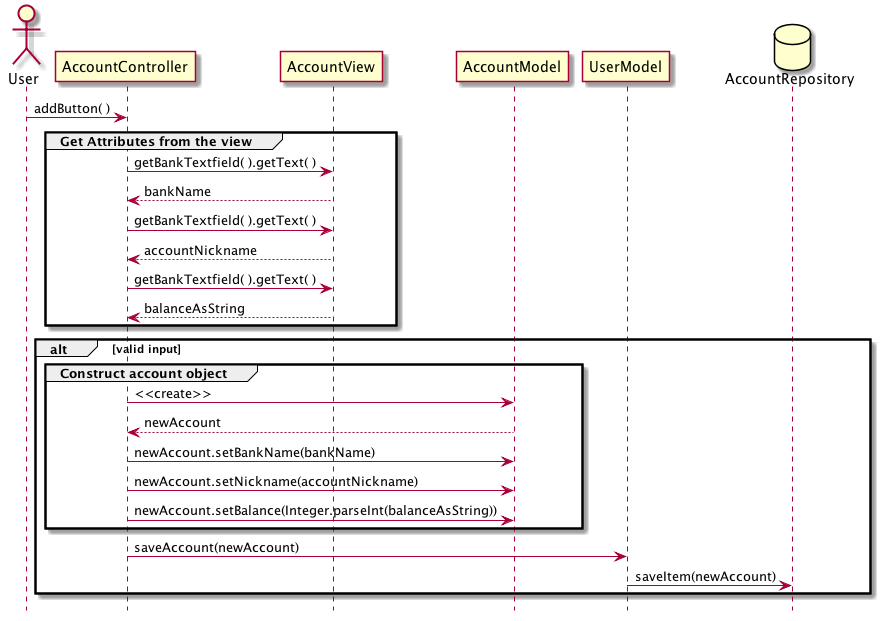
\includegraphics[width=\textwidth,height=\textheight,keepaspectratio]{diagrams/sequence/addAccount.png}
\captionof{figure}{Adding an account}
\bigskip

\subsection{Update an account}
Updating and existing \code{Account} is very similar to creating a new one. The one difference is that the user must first select an entry from the view. The fields will then update to show the selected \code{Account}'s information. The user can then modify the fields as desired and press the "Update" button when ready. The flow is then identical to \ref{sec:addAccount}, with the exception that the \code{AccountController} will set the created \code{Account} object's id from the one selected by the user. Again, the sequence of calls for updating a \code{Transaction} is fundamentally the same.\\
\\
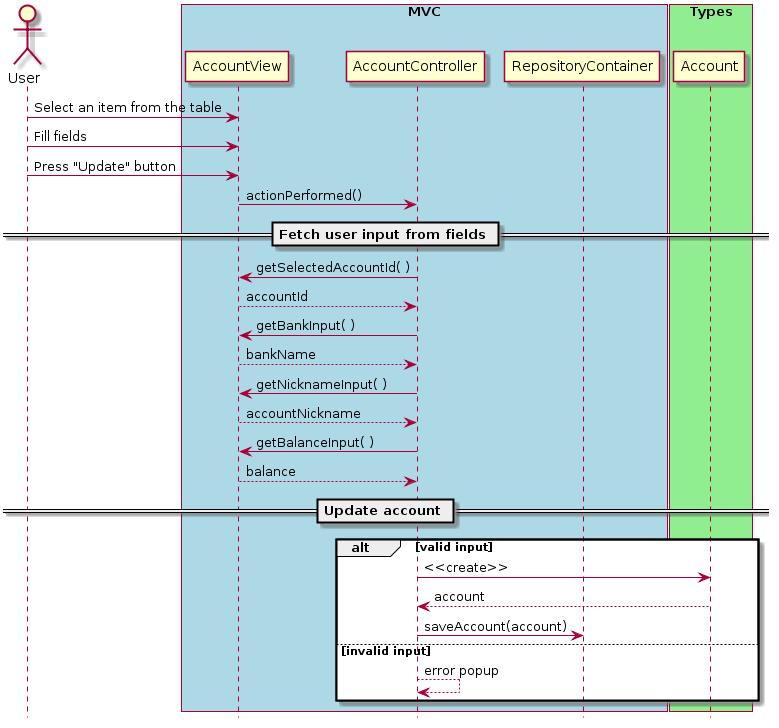
\includegraphics[width=\textwidth,height=\textheight,keepaspectratio]{diagrams/sequence/updateAccount.png}
\captionof{figure}{Updating an account}
\bigskip

\subsection{Delete an account}
To delete an account, the user selects an entry in the \code{AccountView}'s table and clicks the "Delete" button. This sends an \code{ActionEvent} to the \code{AccountController}. The registered listener for this event then calls the \code{deleteAccount()} on the model. \code{Transaction} deletion is handled similarly.\\
\\
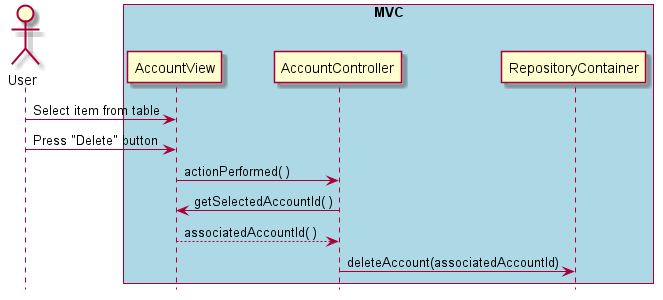
\includegraphics[width=\textwidth,height=\textheight,keepaspectratio]{diagrams/sequence/deleteAccount.png}
\captionof{figure}{Deleting an account}
\bigskip

\newpage
\subsection{Import a transaction list}
In this scenario, the users imports a list of transactions from a .csv file and adds them to the model. When the user clicks the "Import" button, the \code{TransactionController} creates a window with a dialog box. The user then inputs the file path of the transaction csv file. If the file path is valid, both the file path and the currently selected accountId is passed to the model with a call to \code{importTransactions()}. For details on how the model then handles the import, see \ref{sec:modelImportDetail}.\\
\\
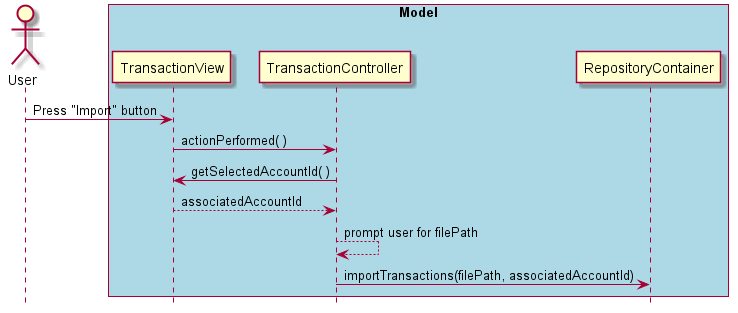
\includegraphics[width=\textwidth,height=\textheight,keepaspectratio]{diagrams/sequence/importHighLevel.png}
\captionof{figure}{Import a list of transactions from .csv file}
\bigskip

\subsection{Model implementation details}
The next subsections offer a glimpse into the internal logic of the model and how it implements the methods of its interface.

\subsubsection{saveAccount()} \label{sec:modelSaveDetail}
The \code{saveAccount(Account)} method provides a simple interface for adding new \code{Account} objects or updating existing ones. When the specified \code{Account} object's \code{accountId} member variable is 0, it is assumed that this is a new entry. Otherwise the call is treated as an update. \\ 

After the \code{saveItem()} method is called, the \code{AccountRepository} creates an \code{SQLValueMap} object (linked HashMap with keys and values of type String) to store the column-value mapping. \\

If the account is new, then the repository uses the \code{SQLStringFactory} class to build a \code{String} insert query using the (key,value) pairs in the \code{SQLValueMap}. It executes the query by calling \code{updateSQL} from the Database class. The repository then updates the account's ID using the accountId value returned from updateSQL and proceeds to add the new account to the repository's \code{AccountMap}.\\

If the account already exists, then the repository will construct a \code{SQLValueMap} for the where clause of the query using the account's ID. \code{SQLStringFactory} is then used to generate an update query, which will be executed by calling the \code{Database} class's \code{updateSQL} method. The returned accountId is unused. \\
\\
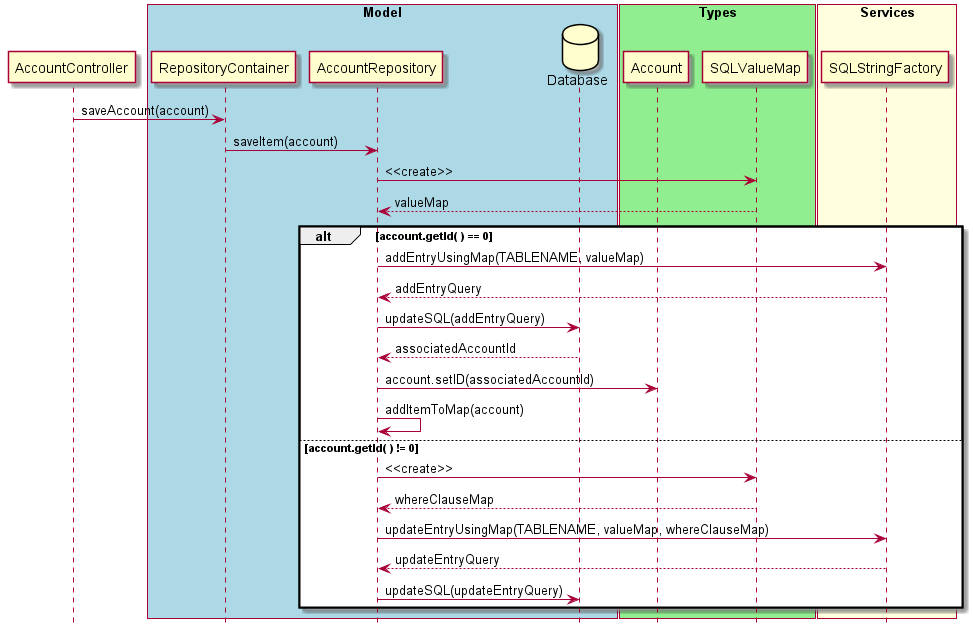
\includegraphics[width=\textwidth,height=\textheight,keepaspectratio]{diagrams/sequence/addAccountImp.png}
\captionof{figure}{Model - Saving an account}
\bigskip

\newpage
\subsubsection{importTransactions()} \label{sec:modelImportDetail}
The \code{importTransaction()} method first creates a \code{BufferedReader} using the file path. Then, it iterates over the file, line by line, using the \code{BufferedReader}'s \code{readLine()} method. \\

The line is split into tokens using the \code{split()} method. Using the returned array of tokens, a \code{Transaction} object is constructed. The model then saves the new\code{Transaction} object by calling its own \code{saveTransaction()} method.\\
\\
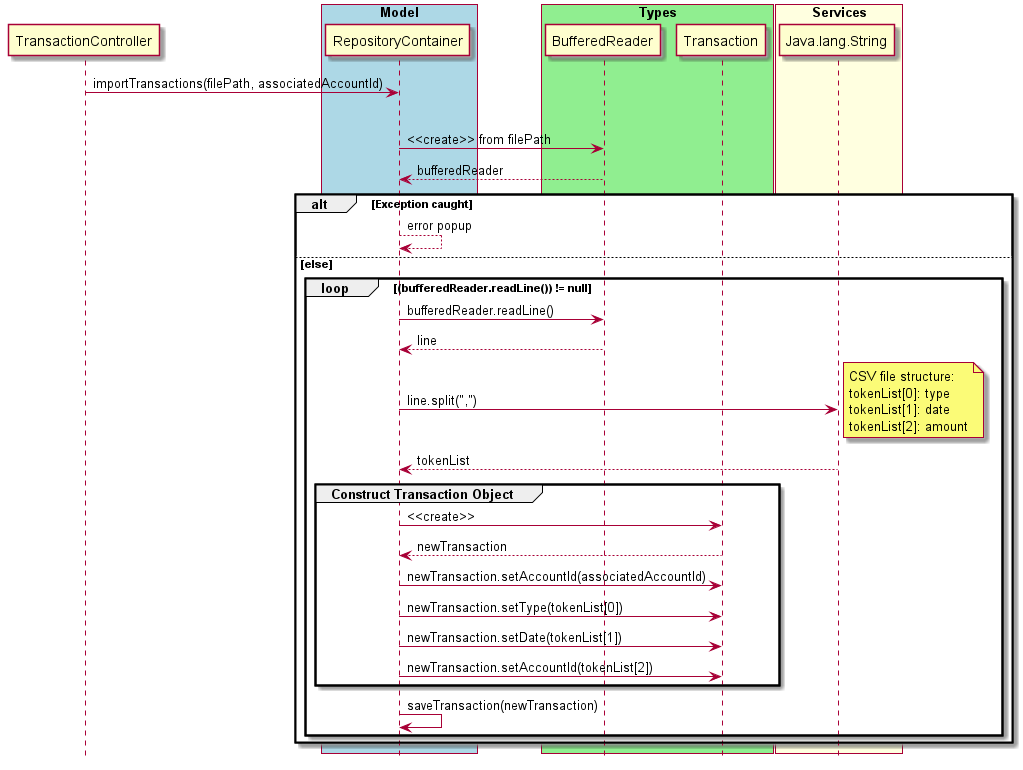
\includegraphics[width=\textwidth,height=\textheight,keepaspectratio]{diagrams/sequence/importLowLevel.png}
\captionof{figure}{Model - Import list of transactions from .csv file}
\bigskip


\end{document}